%FOR PDFLATEX USE ONLY
\documentclass[a4paper,12pt]{article}

\usepackage{amssymb,amsmath} %math symbols

\usepackage[margin=2cm]{geometry} %paper geometry

\usepackage[T1, T2A]{fontenc}

\usepackage[utf8]{inputenc} %allows unicode (including russian) source file
\usepackage[russian]{babel} %docment in russian-style
\usepackage[utf8]{inputenc}
%\usepackage[unicode]{hyperref} %links inside of the text
\usepackage[pdftex]{graphicx} %includegraphics pictures
\usepackage{cmlgc} %bold text

\usepackage{array} %arrays

%\usepackage{wrapfig}
%\usepackage{array}
%\usepackage{lipsum}
%\usepackage{esvect}
%\usepackage{hyperref}

\usepackage{amsmath}
\usepackage{amssymb}
\usepackage{mathtools}
\usepackage{mathtext}

\usepackage{subfig}
%\usepackage{calc}
%\usepackage{pgfplots,tikz,circuitikz}
%\usepackage{tkz-euclide}
\include{wrapfigure}

\begin{document}

\begin{center}
  \LARGE{Работа Д.2.5}\\[0.2cm]
  \LARGE{Определение коэффициента диффузии гелия через резиновую оболочку воздушного шарика}\\[0.2cm]
  \large{Панферов Андрей}\\[0.2cm]
\end{center}  
  
\section{Цель работы:}

Знакомство с явлениями переноса. Определениекоэффициента диффузии гелия через резиновую оболочку воздушного шарика.\\

\section{В работе используются:}

Два одинаковых резиновых шарика шарообразной формы, один из которых накачан гелием, весы, секундомер, небольшой груз (гайка),нитка, ножницы, бумажный метр, миллиметровая бумага.

\section{Аннотация:}

Воздушный шарик, накачанный гелием, со временем достаточно быстро сдувается. Это связано с диффузией гелия через резиновую оболочку шарика. Плотность потока гелия $j$ определяется законом Фика:

\[j = D \Delta n / \delta,\]

где $D$ - коэффициент диффузии гелия через резину, $\delta$ - толщина резиновой оболочки накаченного шарика, $\Delta n = n - n_0$ - разность концентраций гелия внутри и вне шарика.

За время $t$ через всю поверхностьрезиновой оболочкишарика $S$ в атмосферу выйдет:

\[\Delta N = jSt = \frac{DSNt}{\delta V}\]

молекул гелия.\\

Пренебрегая утечкой газа через узел, а также проникновением молекул воздуха внутрь шарикаи, т.е.,предполагая, что оболочка шарика проницаема только для гелия, получим, что относительное изменениевеличины подъёмной силы шарика за время $t$ равно:

\[\Delta F_п = - \frac{DS(\rho_{air} - \rho_{He})gt}{\delta}\]

При этом мы считали, чтодавление гелия внутри шарика незначительно превосходит атмосферное (реально, для шаров шарообразной формы давление в шарике превосходит атмосферное на $\approx$ 5\%).

\newpage

\begin{wrapfigure}{l}{0.18\textwidth}
    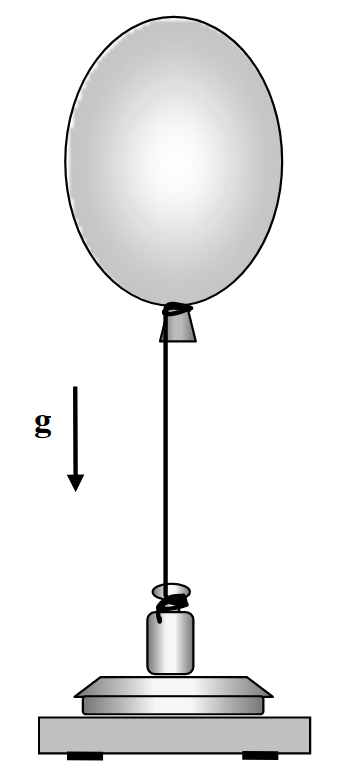
\includegraphics[width=0.18\textwidth]{bal.png}
    \caption{Схема установки}
    \label{fig:bal}
\end{wrapfigure}

\section{Методика измерений:}

Привяжем к нити гелиевого шарика груз и положим груз на весы как показано на рисунке \ref{fig:bal}. Сила тяжести груза превышает подъёмную силу шарика.Сила, действующая на платформу весов, равна:

\[F = m_{гр}g - F_п\]

где $m_{гр}$ - суммарная масса груза и оболочки с ниткой.
Поскольку с течением времени подъёмная сила уменьшается линейно, то показания весов, начиная с некоторого начального значения $m_0$, увеличиваются по линейному закону. Таким образом, коэффициент диффузии $D$ можно определить по значению углового коэффициента $\beta$ графика экспериментальной зависимости $m(t)$ по формуле:
\[D = \beta \delta / S(\rho_{air} - \rho_{He})\]


\section{Данные и их обработка:}

\begin{table}[h!]

\begin{minipage}{0.3\textwidth}
\begin{tabular}{|l|l|}
\hline
t, мин                & m, г                     \\ \hline
0                     & 2.74                     \\ \hline
3                     & 2.78                     \\ \hline
6                     & 2.80                     \\ \hline
9                     & 2.83                     \\ \hline
12                    & 2.84                     \\ \hline
15                    & 2.89                     \\ \hline
18                    & 2.91                     \\ \hline
21                    & 2.95                     \\ \hline
24                    & 2.98                     \\ \hline
27                    & 3.01                     \\ \hline
30                    & 3.03                     \\ \hline
33                    & 3.07                     \\ \hline
36                    & 3.11                     \\ \hline
39                    & 3.15                     \\ \hline
42                    & 3.17                     \\ \hline
45                    & 3.20                     \\ \hline
48                    & 3.22                     \\ \hline
51                    & 3.26                     \\ \hline
54                    & 3.29                     \\ \hline
57                    & 3.31                     \\ \hline
60                    & 3.34                     \\ \hline
$\sigma t \approx$ 1c & $\sigma m \approx$ 0.1г \\ \hline
\end{tabular}
\end{minipage}
\begin{minipage}{0.7\textwidth}
Измерим параметры шарика до надувания: $m = (2.61 \pm 0.4)г$, табличная плотность резины - $1.05 г/см^3$

Геометрические параметры воздушного шарика будем измерять мерной лентой с экспериментальной погрешностью 0.1 см. Его форму приблизим объединением полусферы диаметра $d$ и конуса с длиной стороны $l$.\\

Парамеры шарика до и после эксперимента:
\begin{enumerate}
	$d_1 = 23,62 \pm 0.03см$, $l_1 = 25.0 \pm 0.2см$,\\
	$V_0 = \pi d^2(d + \sqrt{l^2 - (d/2)^2}) / 12 = (66.7 \pm 0.3) \cdot 10 ^ {2} \:\:см^3$,\\
	$d_1 = 23,21 \pm 0.03см$, $l_1 = 24.2 \pm 0.2см$,\\
	$V_1 = \pi d^2(d + \sqrt{l^2 - (d/2)^2}) / 12 = (62.6 \pm 0.3) \cdot 10 ^ {2} \:\:см^3$,\\
	$S = (1804 \pm 8) см^2$, $\delta = \frac{m}{\rho S} = (13.8 \pm 0.2)мкм$
\end{enumerate}
Как мы видим, $\frac{V_0 - V_1}{V_0} \approx 6\%$, что в пределах наших приближений. Параметры окружающей среды:
\begin{enumerate}
	$\rho_{air} = (120.3 \pm 0.4) \cdot 10^{-2}кг/м^3$,\\
	$\rho_{He} = (17.8 \pm 0.1) \cdot 10^{-2}кг/м^3$,\\
	$p = 101.5 кПа$,\\
	$T = (295 \pm 1) К$

\end{enumerate}

\end{minipage}
\end{table}

\begin{tikzpicture}[scale=1.5]
	\begin{axis}[
		axis lines = left,
    	xlabel = {t, мин},
    	ylabel = {m, г},
    	ylabel style={black, scale=0.7},
    	xlabel style={black, scale=0.7},
    	%xmin=0, xmax=9,
    	title={Зависимость $m$ от $t$},
    	legend style={at={(0.03,-0.4)},anchor=west}
		]
		\addplot+[blue, only marks]  plot[
			error bars/.cd,
			y dir=both,
			y fixed = 0.1,
		]
		coordinates
		{(0, 2.74) (3, 2.78) (6, 2.80) (9, 2.83) (12, 2.84) (15, 2.89) (18, 2.91) (21, 2.95) (24, 2.98) (27, 3.01) (30, 3.03) (33, 3.07) (36, 3.11) (39, 3.15) (42, 3.17) (45, 3.20) (48, 3.22) (51, 3.26) (54, 3.29) (57, 3.31) (60, 3.34)};
		\addplot[color=red, domain=0:60]{2.74 + 0.0102 * x};
		

	\end{axis}
\end{tikzpicture}

Методом наименьших квадратов найдем угловой коэффициент графика $m(t)$:
\[\beta = (1.70 \pm 0.12) \cdot 10^{-7} кг/с\]

И из него находим $D$:

\[D = \frac{\beta \delta}{S(\rho_{ait} - \rho_{He})} = (1.25 \pm 0.09) \cdot 10^{-11}\frac{м}{с^2}\]

\section{Вывод:}

Получен коэффициент диффузии гелия через резину. Основной вклад в погрешность внесли измерения массы (порядка 4\%).\\

Учитывая приближения, сделанные в данном эксперименте, такие как \textbf{Принебрежение изменением площади поверхности шарика($\approx$4 \%)}, \textbf{Пренебрежение добавочным давлением в шарике ($\approx$3 \%)}, можно модифицировать погрешность итогового результата и получить:
\[D = (1.25 \pm 0.11)\cdot 10^{-11}\frac{м}{с^2}\] 

\textbf{Оценим коэффициент диффузии воздуха через резину}, используя данные об изменении объема шарика:
\[\frac{|\Delta F|}{g} = (0.60 \pm 0.06)г\]
\[\Delta V = V_0 - V_1 = (406 \pm 60 )см^3 \]
Это позволяет нам оценить количество воздуха, проникшего внутрь шарика, и из него - коэффициент диффузии:
\[D_{air} \approx 10^{-14} \sim 10^{-13} \:\:м^2/с\],

что на порядки меньше коэффициента для гелия. Что означает, что приближение, что оболочка непроницаема для воздуха - оправдано.


\end{document}


